\documentclass[portrait]{seminar}
%\usepackage{pandora}
\usepackage{color}
\usepackage{fancybox}
\usepackage{alltt}
\usepackage{epsfig}
\usepackage{rail}
\usepackage{bar}
\usepackage{url}
\usepackage{rotating}
\usepackage[normalem]{ulem}
\usepackage{latexsym}
\usepackage{amsmath}

\begin{document}

\boldmath
\newcommand{\RA}{$\rightarrow$}
\newcommand{\LL}{\mbox{$[$\hspace{-0.15em}$[$}}
\newcommand{\RR}{\mbox{$]$\hspace{-0.15em}$]$}}
\newcommand{\CC}[1]{\mbox{\tt $\LL$#1$\RR$}}

\slideframe{shadow}

%%% Activate one of these to get either Aarhus style or McGill style 
%%% by putting a #1 in the appropriate line.
\newcommand{\mcgill}[1]{#1}
\newcommand{\aarhus}[1]{}

%%% Define this to be the name of your term
\newcommand{\courseterm}{Fall 2012}




\aarhus{
\newpagestyle{dOvsstyle}{dOvs'98 Week 40 \hfil The WIG language}{\hfil \thepage}
}

\mcgill{
\newpagestyle{dOvsstyle}{ COMP 520 \courseterm  \hfil The WIG language (\thepage)}{}
}
 
\slidepagestyle{dOvsstyle}

\begin{slide*}
\begin{tabbing}
\aarhus{{\Large\bf Week 40}\\}
~\\
{\Huge\bf The}\\ ~\\
\psfig{file=wig.EPSF,width=4cm}\\ ~\\{\Huge\bf language}\\
\end{tabbing}
\vfil
\end{slide*}

\begin{slide*}
Uses of the World Wide Web:
\begin{itemize}
\item static documents\\(supported by HTML);
\item dynamic documents\\(supported by CGI, ASP, Ruby on Rails, various HTML
extensions, \ldots); and
\item interactive services\\(supported by \verb"<bigwig>" and MAWL).
\end{itemize}
\vfil
\end{slide*}
 
\begin{slide*}
Static documents:
\begin{itemize}
\item there are too many documents;
\item the documents are rarely updated; and
\item the documents are not customized.
\end{itemize}
\vspace*{2ex}

Dynamic documents:
\begin{itemize}
\item there are fewer documents;
\item the documents are always updated;
\item the documents are customized.
\end{itemize}
\vfil
\end{slide*}
 
\begin{slide*}
Standard interaction:

\begin{center}
\setlength{\unitlength}{0.000600in}%
%
\begingroup\makeatletter\ifx\SetFigFont\undefined%
\gdef\SetFigFont#1#2#3#4#5{%
  \reset@font\fontsize{#1}{#2pt}%
  \fontfamily{#3}\fontseries{#4}\fontshape{#5}%
  \selectfont}%
\fi\endgroup%
\begin{picture}(4824,2064)(1489,-3313)
\thicklines
\put(4801,-3061){\framebox(1500,1800){}}
\put(1501,-3061){\framebox(1500,1800){}}
\put(3001,-1711){\vector( 1, 0){1800}}
\put(5101,-2011){\vector(-1, 0){2100}}
\put(5101,-2161){\framebox(900,750){}}
\put(5326,-3286){\makebox(0,0)[lb]{\smash{\SetFigFont{8}{14.4}{\familydefault}{\mddefault}{\updefault}Server}}}
\put(1951,-3286){\makebox(0,0)[lb]{\smash{\SetFigFont{8}{14.4}{\familydefault}{\mddefault}{\updefault}Client}}}
\put(3751,-1636){\makebox(0,0)[lb]{\smash{\SetFigFont{8}{14.4}{\familydefault}{\mddefault}{\updefault}URL}}}
\put(3276,-2186){\makebox(0,0)[lb]{\smash{\SetFigFont{8}{14.4}{\familydefault}{\mddefault}{\updefault}static document}}}
\put(5226,-1861){\makebox(0,0)[lb]{\smash{\SetFigFont{8}{14.4}{\familydefault}{\mddefault}{\updefault}HTML}}}
\end{picture}
\end{center}
~\\

Common Gateway Interface:
\begin{center}
\setlength{\unitlength}{0.0006in}%
%
\begingroup\makeatletter\ifx\SetFigFont\undefined%
\gdef\SetFigFont#1#2#3#4#5{%
  \reset@font\fontsize{#1}{#2pt}%
  \fontfamily{#3}\fontseries{#4}\fontshape{#5}%
  \selectfont}%
\fi\endgroup%
\begin{picture}(4824,2064)(1489,-3313)
\thicklines
\put(4801,-3061){\framebox(1500,1800){}}
\put(1501,-3061){\framebox(1500,1800){}}
\put(3001,-1711){\vector( 1, 0){1800}}
\put(5101,-2011){\vector(-1, 0){2100}}
\put(5101,-2161){\framebox(900,750){}}
\put(5101,-2911){\framebox(900,600){}}
\put(3001,-2536){\vector( 1, 0){2100}}
\put(5101,-2686){\vector(-1, 0){2100}}
\put(5326,-3286){\makebox(0,0)[lb]{\smash{\SetFigFont{8}{14.4}{\familydefault}{\mddefault}{\updefault}Server}}}
\put(1951,-3286){\makebox(0,0)[lb]{\smash{\SetFigFont{8}{14.4}{\familydefault}{\mddefault}{\updefault}Client}}}
\put(3751,-1636){\makebox(0,0)[lb]{\smash{\SetFigFont{8}{14.4}{\familydefault}{\mddefault}{\updefault}URL}}}
\put(5226,-1861){\makebox(0,0)[lb]{\smash{\SetFigFont{8}{14.4}{\familydefault}{\mddefault}{\updefault}HTML}}}
\put(5326,-2686){\makebox(0,0)[lb]{\smash{\SetFigFont{8}{14.4}{\familydefault}{\mddefault}{\updefault}script}}}
\put(3406,-2191){\makebox(0,0)[lb]{\smash{\SetFigFont{8}{14.4}{\familydefault}{\mddefault}{\updefault}fill-out form}}}
\put(3551,-2481){\makebox(0,0)[lb]{\smash{\SetFigFont{8}{14.4}{\familydefault}{\mddefault}{\updefault}form data}}}
\put(3086,-2856){\makebox(0,0)[lb]{\smash{\SetFigFont{8}{14.4}{\familydefault}{\mddefault}{\updefault}dynamic document}}}
\end{picture}
\end{center}
\vfil
\end{slide*}
 
\begin{slide*}
Fill-out forms are HTML elements.\\

The \verb"<form ...>" tag contains:
\begin{itemize}
\item the transmission method ({\tt POST} or {\tt GET});
\item the URL of the script; and
\item a query string.
\end{itemize}
\vspace*{2ex}

Extra tags for input fields:
\begin{itemize}
\item simple text fields;
\item radio buttons;
\item menus; and
\item submit buttons.
\end{itemize}
\vfil
\end{slide*}
 
\begin{slide*}
A simple fill-out form:\\

\begin{center}

\psfig{file=form.eps,width=18em}
\end{center}
\vfil
\end{slide*}
 
\begin{slide*}
HTML source for the fill-out form:

\begin{scriptsize}
\begin{verbatim}

<form 
   method="POST" 
   action="http://www.brics.dk/cgi-mis/Python?Questions"
>
Your name: 
<input name="name" type="text" size=20>.
<p>
Your quest:
<select name="quest">
<option value="grail">to find the Holy Grail
<option value="wig">to write a WIG compiler
</select>
<p>
Your favorite color:
<input name="color" type="radio" value="red">red
<input name="color" type="radio" value="green">green
<input name="color" type="radio" value="blue">blue
<input name="color" type="radio" value="argh">I don't know
<p>
<input name="submit" type="submit" value="Answer">
</form>

\end{verbatim}
\end{scriptsize}
\vfil
\end{slide*}

\begin{slide*}
After filling out the form and clicking on the submit button, your browser
sends the following text to the web server:\\

\begin{scriptsize}
\begin{verbatim}
POST /cgi-mis/Python?Questions HTTP/1.0
Accept: www/source
Accept: text/html
......
User-Agent: ...  ...
From: ...
Content-type: application/x-www-form-urlencoded
Content-length: 47

name=Michael
&quest=wig
&color=blue
&submit=Answer
\end{verbatim}
\end{scriptsize}
\vfil
\end{slide*}

\begin{slide*}
The web server parses the data from the client (e.g., a browser), 
sets environment variables and input, and invokes CGI scripts.

Additional information is available in several UNIX environment
variables.  Consider the following simple query

{\scriptsize
  \verb+http://www.cs.mcgill.ca/~hendren/cgi-bin/myenv.cgi?foo+} :\\

\begin{scriptsize}
\begin{verbatim}
QUERY_STRING = foo 
SERVER_ADDR = 132.206.51.10
HTTP_ACCEPT_LANGUAGE = en-us,en;q=0.5
SERVER_PROTOCOL = HTTP/1.1
HTTP_CONNECTION = keep-alive
REMOTE_PORT = 35406
HTTP_USER_AGENT = 
  Mozilla/5.0 (X11; U; Linux i686; en-US; rv:1.4)
  Gecko/20030624
HTTP_ACCEPT = text/xml,application/xml,application/xhtml+xml,
              text/html;q=0.9,text/plain;q=0.8,video/x-mng,
              image/png,image/jpeg,image/gif;q=0.2,*/*;q=0.1
GATEWAY_INTERFACE = CGI/1.1
HTTP_HOST = www.cs.mcgill.ca
SERVER_ADMIN = help@cs.mcgill.ca
SERVER_SOFTWARE = Apache/2.0.43 (Unix) PHP/4.3.0RC2
SCRIPT_URI = 
  http://www.cs.mcgill.ca/~hendren/cgi-bin/myenv.cgi
REMOTE_ADDR = 132.206.3.136
SCRIPT_NAME = /~hendren/cgi-bin/myenv.cgi
SCRIPT_URL = /~hendren/cgi-bin/myenv.cgi
HTTP_ACCEPT_ENCODING = gzip,deflate
SERVER_NAME = www.cs.mcgill.ca
DOCUMENT_ROOT = /usr/local/www/data
REQUEST_URI = /~hendren/cgi-bin/myenv.cgi?Questions
HTTP_ACCEPT_CHARSET = ISO-8859-1,utf-8;q=0.7,*;q=0.7
REQUEST_METHOD = GET
SCRIPT_FILENAME = 
  /u0/prof/hendren/public_html/cgi-bin/myenv.cgi
HTTP_KEEP_ALIVE = 300
PATH = /usr/local/bin:/usr/local/bin:/usr/bin:/bin
SERVER_PORT = 80
\end{verbatim}
\end{scriptsize}
\vfil
\end{slide*}

\begin{slide*}
The script may be written in any programming or scripting language.\\

The form data appears on standard input as:

\begin{scriptsize}
\begin{verbatim}
 
name=Michael&quest=wig&color=blue&submit=Answer

\end{verbatim}
\end{scriptsize}

but must first be decoded:
\begin{itemize}
\item change \verb:'+': into a space character; and
\item replace \verb:%xy: by the ASCII character with hex value \verb"xy".
\end{itemize}

In this example, \verb"'='" and \verb"'&'" must be encoded.

For more on URL encoding see:\\
{\scriptsize\url{http://www.w3schools.com/HTML/html_urlencode.asp}} 
\vfil
\end{slide*}
 

\begin{slide*}
\newcommand{\important}{\hspace*{15em}$\longleftarrow${\rm\em important blank line}}
The dynamic document is supplied by the script on standard output:

\begin{scriptsize}
\begin{alltt}
 
Content-type: text/html
\important{}
Hello Michael,
<p>
Good luck on writing a blue WIG compiler!

\end{alltt}
\end{scriptsize}

or may be redirected from a different document:

\begin{scriptsize}
\begin{verbatim}

Location: http://some.abolute/url
Content-type: text/html

\end{verbatim}
\end{scriptsize}

How do we know it is really HTML?

%We don't...
\vfil
\end{slide*}
 
\begin{slide*}
CGI is a state-less protocol:
\begin{itemize}
\item each exchange happens in isolation;
\item no information remains on the server; and
\item different users cannot communicate.
\end{itemize}
\vspace*{2ex}

We would like to have:
\begin{itemize}
\item global state;
\item sessions;
\item concurrent threads; and
\item local state.
\end{itemize}

\vfil
\end{slide*}
 
\begin{slide*}
Interacting with a service:\\


\psfig{file=play1.eps,width=10.2em}

\psfig{file=play2.eps,width=10.2em}

\psfig{file=play3.eps,width=10.2em}

\psfig{file=play4.eps,width=10.2em}

\psfig{file=play5.eps,width=10.2em}

\psfig{file=play6.eps,width=10.2em}\\

\psfig{file=play7.eps,width=20.7em}\\

\psfig{file=play8.eps,width=10.2em}
\vfil
\end{slide*}
 
\begin{slide*}
\vfil
\end{slide*}
 
\begin{slide*}
The WIG language provides:

\begin{itemize}
\item global state;
\item safe, dynamic documents;
\item sequential sessions;
\item multiple threads; and
\item local state.
\end{itemize}
\vspace*{2ex}

A WIG specification is compiled into a self-contained CGI-script.
\vfil
\end{slide*}

\begin{slide*}
The (once) ubiquitous counter:

\begin{scriptsize}
\begin{verbatim}
service {
  const html Nikolaj = <html> <body>
     <img src="http://www.brics.dk/~mis/babybath.jpg">
     <p>
     <i>You are visitor number <[no]></i>
  </body> </html>;

  int counter;

  session Access() {
    counter = counter + 1;
    exit plug Nikolaj[no = counter];
  }
}
\end{verbatim}
\end{scriptsize}
\begin{center}
\aarhus{
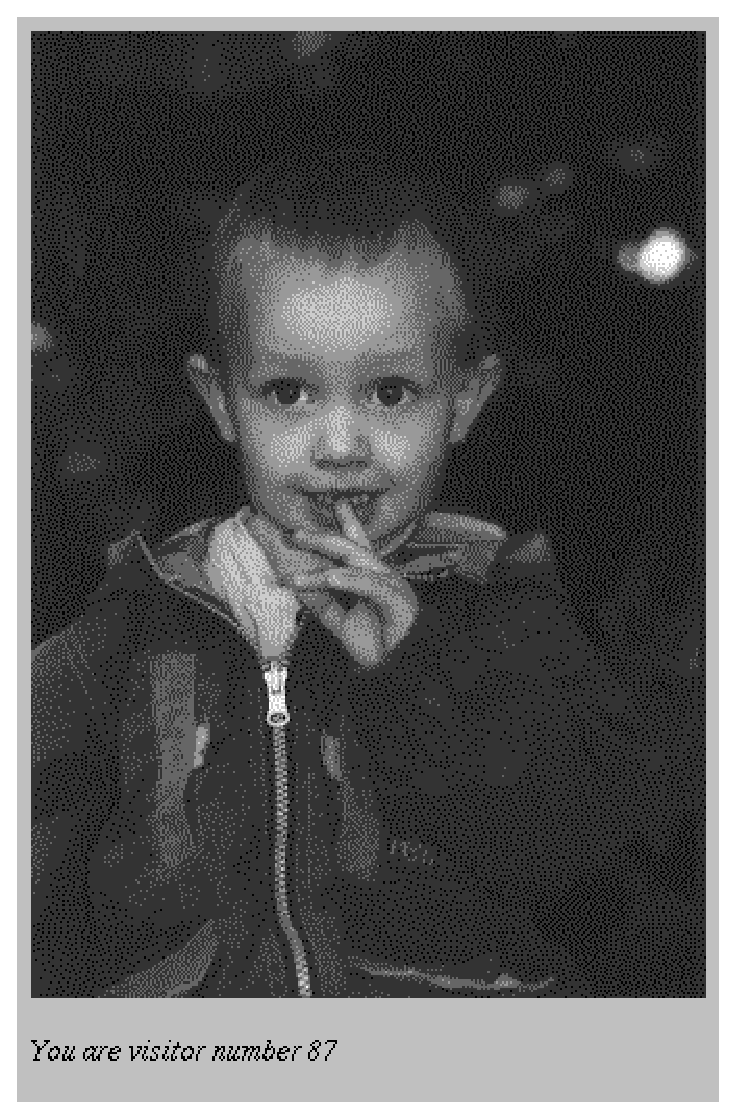
\epsfig{file=nikolaj.eps,height=15em}
}
\mcgill{
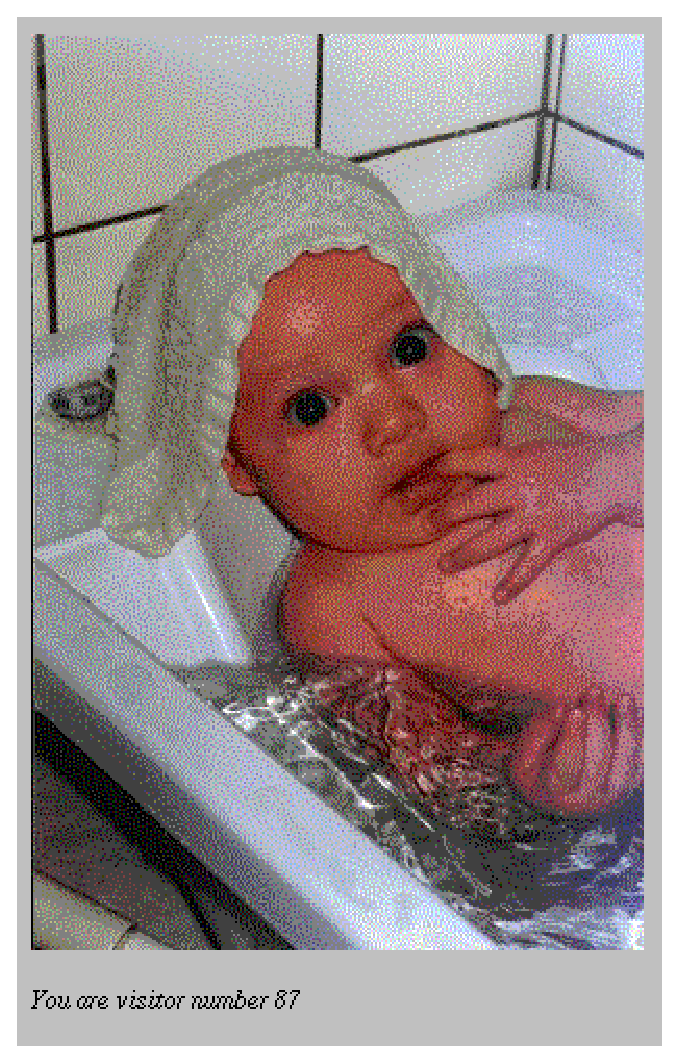
\epsfig{file=babybath.eps,height=15em}
}
\end{center}

\vfil
\end{slide*}

\begin{slide*}
A one-player guessing game:

\begin{scriptsize}
\begin{verbatim}
service {
  const html GetSeed = <html> <body> ... </body> </html>;
  const html GameSeeded = <html> <body> ... </body> </html>;
  const html Init = <html> <body> ... </body> </html>;
  const html Retry = <html> <body> ... </body> </html>;
  const html Again = <html> <body> ... </body> </html>; 
  const html Done = <html> <body> ... </body> </html>; 
  const html Record = <html> <body> ... </body> </html>;
  const html Finish = <html> <body> ... </body> </html>;
  const html List = <html> <body> ... </body> </html>; 

  int plays, record;
  int seed;
  string holder;

  int nextRandom() {
    int current;
    
    seed = (25173 * seed + 13849) % 65536;
    return(seed); 
  } 
  
  session Seed() {
    show GetSeed receive[seed = seed];
    exit GameSeeded;
  } 

  ...
}
\end{verbatim}
\end{scriptsize}
\vfil
\end{slide*}
 
\begin{slide*}
\begin{scriptsize}
\begin{verbatim}
  session Play() {
    int number, guesses, guess;
    string localholder;
    
    number = nextRandom() % 100;
    plays = plays + 1;
    guesses = 1;
    show Init receive[guess = guess];
    while (guess > 99) show Retry receive[guess = guess];
    while (guess != number) {
      guesses = guesses + 1;
      if (guess > number) 
        show plug Again[correction = "lower"] 
          receive[guess = guess];
      else
        show plug Again[correction = "higher"] 
          receive[guess = guess];
      while (guess > 99) show Retry receive[guess = guess];
    }  
    show plug Done[trys = guesses];
    if (record == 0 || record > guesses) {
      show plug Record[old = record] 
        receive [localholder = name];
      holder = localholder;
      record = guesses;
    }  
    exit Finish;
  } 
  
  session HiScore() {
    exit plug List[plays = plays,
      holder = holder, record = record];
  } 
\end{verbatim}
\end{scriptsize}
\vfil
\end{slide*}

\begin{slide*}
\begin{scriptsize}
\begin{verbatim}
  const html GetSeed = <html> <body>
    Please enter an integer seed for the random 
    number generator:
    <input name="seed" type="text" size=5>
  </body> </html>;
  
  const html GameSeeded = <html> <body>
    Ok, now the game can proceed, the generator is seeded.
  </body> </html>;
    
  const html Init = <html> <body>
    Please guess a number between 0 and 99:
    <input name="guess" type="text" size=2>
  </body> </html>;
    
  const html Retry = <html> <body>
    That number is too large!
    <p> 
    Please keep your guess between 0 and 99:
    <input name="guess" type="text" size=2>
  </body> </html>;
  
  const html Again = <html> <body>
    That is not correct. Try a <[correction]> number:
    <input name="guess" type="text" size=2>
  </body> </html>;
\end{verbatim}
\end{scriptsize}
\vfil
\end{slide*}
 
\begin{slide*}
\begin{scriptsize}
\begin{verbatim}
  const html Again = <html> <body>
    That is not correct. Try a <[correction]> number:
    <input name="guess" type="text" size=2>
  </body> </html>; 
   
  const html Done = <html> <body>
    You got it, using <[trys]> guesses.
  </body> </html>; 
     
  const html Record = <html> <body>
    That makes you the new record holder,
    beating the old record of <[old]> guesses.
    <p>
    Please enter your name for the hi-score list
    <input name="name" type="text" size=20>
  </body> </html>; 
    
  const html Finish = <html> <body>
    Thanks for playing this exciting game.
  </body> </html>; 
   
  const html List = <html> <body>
    In <[plays]> plays of this game, the record
    holder is <[holder]> with <[record]> guesses.
  </body> </html>; 
\end{verbatim}
\end{scriptsize}
\vfil
\end{slide*}
 
\begin{slide*}
Syntax for WIG html:

\begin{scriptsize}
\begin{verbatim}
htmls : html | htmls html ;
html : "const" "html" identifier "=" 
       "<html>" htmlbodies "</html>" ;

htmlbodies : /* empty */ | nehtmlbodies;
nehtmlbodies : htmlbody | nehtmlbodies htmlbody;
htmlbody : "<" identifier attributes ">"
         | "</" identifier ">"
         | "<[" identifier "]>"
         | whatever
         | meta
         | "<" "input" inputattrs ">"
         | "<" "select" inputattrs ">" htmlbodies 
           "</" "select" ">";

inputattrs : inputattr | inputattrs inputattr;
inputattr : "name" "=" attr
          | "type" "=" inputtype
          | attribute;
inputtype : "text" | "radio";

attributes : /* empty */ | neattributes;
neattributes : attribute | neattributes attribute;
attribute : attr | attr "=" attr;
attr : identifier | stringconst;
\end{verbatim}
\end{scriptsize}
\vfil
\end{slide*}
 
\begin{slide*}
Comments on WIG html:
\begin{itemize}
\item documents are implicitly forms;
\item the \verb:<[foo]>: tag defines gaps to be filled in dynamically;
\item {\tt <input...>} and {\tt <select...>} tags are explicitly recognized; and
\item all other tags and plain text are permitted but ignored.
\end{itemize}
\vfil
\end{slide*}
 
\begin{slide*}
Syntax for WIG statements:
 
\begin{scriptsize}
\begin{verbatim}
stms : /* empty */ | nestms;
;
nestms : stm | nestms stm
;
stm : ";"
    | "show" document receive ";"
    | "exit" document ";"
    | "return" ";"
    | "return" exp ";"
    | "if" "(" exp ")" stm
    | "if" "(" exp ")" stm "else" stm
    | "while" "(" exp ")" stm
    | compoundstm
    | exp ";"
;
document : identifier
         | "plug" identifier "[" plugs "]";

receive : /* empty */
        | "receive" "[" inputs "]";

compoundstm : "{" variables stms "}";

plugs : plug | plugs "," plug;

plug : identifier = exp;

inputs : /* empty */ | neinputs;
neinputs : input | neinputs "," input;
input : lvalue = identifier;
\end{verbatim}
\end{scriptsize}
\vfil
\end{slide*}
 
\begin{slide*}
Syntax for WIG expressions:
 
\begin{scriptsize}
\begin{verbatim}
exp : lvalue
    | lvalue "=" exp
    | exp "==" exp
    | exp "!=" exp
    | exp "<" exp
    | exp ">" exp
    | exp "<=" exp
    | exp ">=" exp
    | "!" exp
    | "-" exp
    | exp "+" exp
    | exp "-" exp
    | exp "*" exp
    | exp "/" exp
    | exp "%" exp
    | exp "&&" exp
    | exp "||" exp
    | exp "<<" exp
    | exp "\+" identifiers
    | exp "\-" identifiers         
    | identifier "(" exps ")"
    | intconst
    | "true"
    | "false"
    | stringconst
    | "tuple" "{" fieldvalues "}"
    | "(" exp ")"                 
;
\end{verbatim}
\end{scriptsize}
\vfil
\end{slide*}

\begin{slide*}
Syntax for WIG expressions (cont.):
 
\begin{scriptsize}
\begin{verbatim}
exps : /* empty */ | neexps;
neexps : exp | neexps "," exp;

lvalue : identifier | identifier "." identifier;

fieldvalues : /* empty */ | nefieldvalues ;
nefieldvalues : fieldvalue | fieldvalues "," fieldvalue ;
fieldvalue : identifier "=" exp;
\end{verbatim}
\end{scriptsize}
\vfil
\end{slide*}

\begin{slide*}
Syntax for WIG schemas, types and functions:

\begin{scriptsize}
\begin{verbatim}
schemas: /* empty */ | neschemas;
neschemas: schema | neschemas schema;
schema : "schema" identifier "{" fields "}";

fields : /* empty */ | nefields;
nefields : field | nefields field;
field : simpletype identifier ";";

simpletype : "int" | "bool" | "string" | "void";
type : simpletype | "tuple" identifier;

functions : /* empty */ | nefunctions;
nefunctions : function | nefunctions function;
function : type identifier "(" arguments ")" compoundstm;

arguments : /* empty */ | nearguments;
nearguments : argument | nearguments "," argument;
argument : type identifier;
\end{verbatim}
\end{scriptsize}
\vfil
\end{slide*}

\begin{slide*}
Syntax for WIG sessions, variables, and services:

\begin{scriptsize}
\begin{verbatim}
sessions : session | sessions session;
session : "session" identifier "(" ")" compoundstm;

variables : /* empty */ | nevariables ;
nevariables : variable | nevariables variable ;
variable : type identifiers ";" ;
identifiers : identifier | identifiers "," identifier ;

service : "service" "{" htmls schemas 
               variables functions sessions "}" ;
\end{verbatim}
\end{scriptsize}

\vspace{0.2in}

Compare our initial attempt at a grammar with a proper yacc/bison
grammar with all conflicts resolved:

\begin{scriptsize}
\begin{verbatim}
$ diff -u wiggrammar.txt wiggrammar_bison.txt
\end{verbatim}
\end{scriptsize}

\vfil
\end{slide*}
 
\begin{slide*}
Some open questions on WIG semantics:

\begin{itemize}
\item what happens if not all gaps are plugged?
\item what happens if a gap is plugged twice?
\item must all form inputs be received?
\item what are the allowed operations on tuples?
\item what are the type rules?
\item are global variables safe for concurrent threads?
\end{itemize}
\vspace*{2ex}

There are many such questions to ponder.
\vfil
\end{slide*}
 
\begin{slide*}
A simple chat room:

\begin{scriptsize}
\begin{verbatim}
service {  
  const html Logon = <html> <body>
    <h1>Welcome to The Chat Room</h1>    
    Please enter your on-line name:
    <input name="name" type="text" size=25>
  </body> </html>;

  const html Update = <html> <body>
    <h1>The Chat Room Service</h1>    <hr>
    <b>Messages so far:</b>    <p>
    <[msg0]><p><[msg1]><p><[msg2]><p><[msg3]><p>
    <[msg4]><p><[msg5]><p>
    <hr>
    <b>Your new message:</b>
    <p>
    <input name="msg" type="text" size=40>
    <p>
    <hr>
    <p>
    <input name="quit" type="radio" value="yes"> Quit now
  </body> </html>;

  const html ByeBye = <html> <body>
    <h1>Thanks for using The Chat Room</h1>
    You made <[conns]> connections
    and wrote <[msgs]> messages.
  </body> </html>;

  string msg0,msg1,msg2,msg3,msg4,msg5;
\end{verbatim}
\end{scriptsize}
\vfil
\end{slide*}

\begin{slide*}
A simple chat room (cont.):
\begin{scriptsize}
\begin{verbatim}
  session Chat() {
    string name,msg,quit;
    int connections, written;
    
    show Logon receive [name = name];
    while (quit!="yes") {
      show plug Update[msg0 = msg0,
                       msg1 = msg1,
                       msg2 = msg2,
                       msg3 = msg3,
                       msg4 = msg4,
                       msg5 = msg5]
      receive[msg = msg, quit = quit];
      connections = connections+1;
      if (msg!="") {
        written = written+1;
        msg0 = msg1;
        msg1 = msg2;
        msg2 = msg3;
        msg3 = msg4;
        msg4 = msg5;
        msg5 = name + "> " + msg;
      }
    }
    exit plug ByeBye[conns = connections,
                     msgs = written];
  }
}
\end{verbatim}
\end{scriptsize}
\vfil
\end{slide*}

\begin{slide*}
A sample chat:\\

\begin{center}
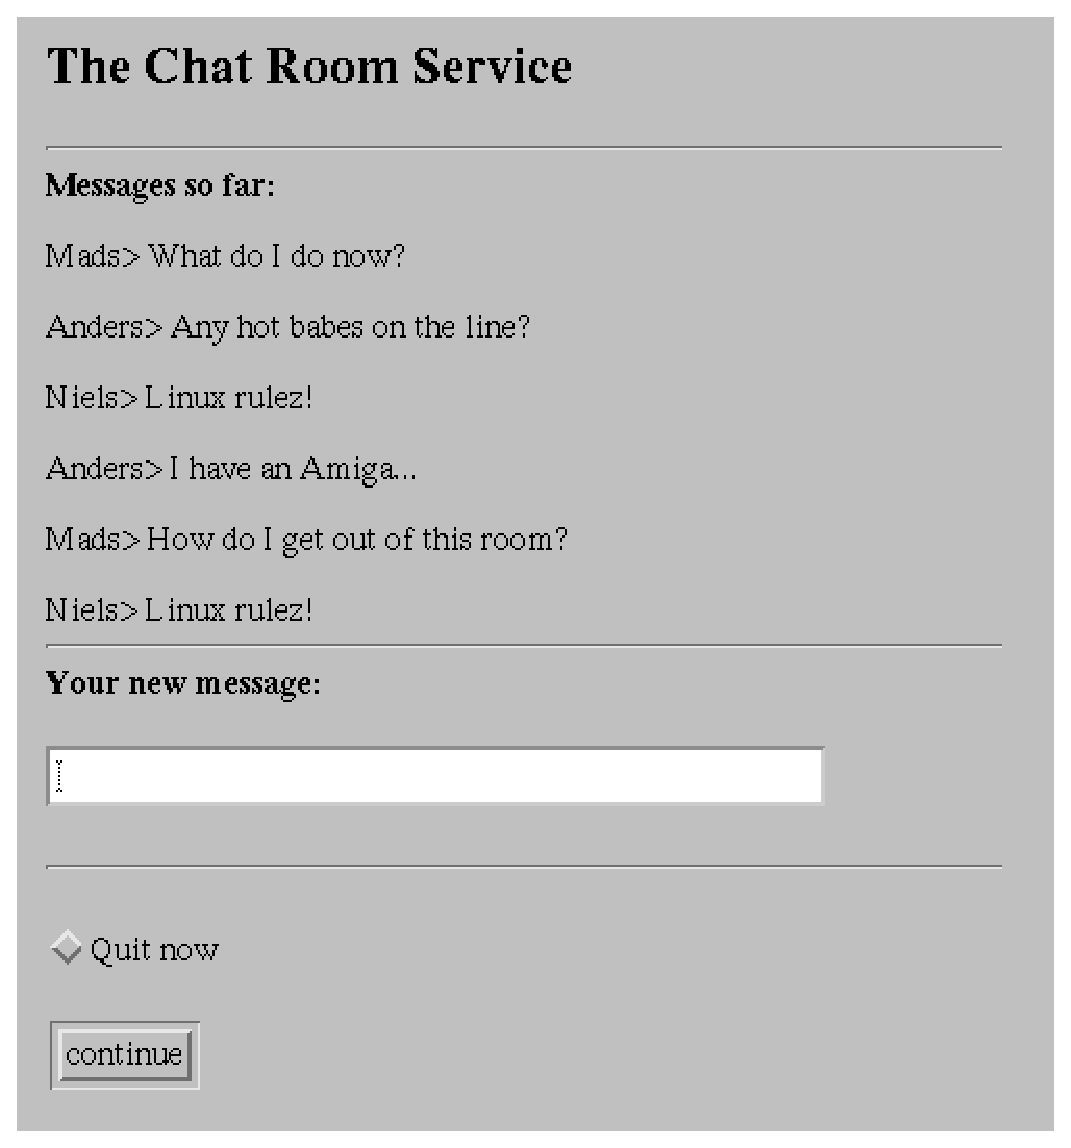
\psfig{file=chat.eps,width=40ex}
\end{center}
\vfil
\end{slide*}

\begin{slide*}
Concurrent threads in a service:\\

\begin{center}
\setlength{\unitlength}{3000sp}%
%
\begingroup\makeatletter\ifx\SetFigFont\undefined%
\gdef\SetFigFont#1#2#3#4#5{%
  \reset@font\fontsize{#1}{#2pt}%
  \fontfamily{#3}\fontseries{#4}\fontshape{#5}%
  \selectfont}%
\fi\endgroup%
\begin{picture}(3634,4524)(2389,-4273)
\thinlines
\put(2401,-1561){\framebox(1200,600){}}
\put(2401,-2761){\framebox(1200,600){}}
\put(2401,-3961){\framebox(1200,600){}}
\thicklines
\put(3601,-1036){\line( 1, 0){900}}
\put(3601,-1111){\line( 1, 0){1200}}
\put(3901,-1261){\line( 1, 0){2100}}
\put(4201,-1336){\line( 1, 0){900}}
\put(3976,-1486){\line( 1, 0){1500}}
\put(3601,-2236){\line( 1, 0){1800}}
\put(3601,-2311){\line( 1, 0){2100}}
\put(3901,-2461){\line( 1, 0){1200}}
\put(3676,-2536){\line( 1, 0){1725}}
\put(4501,-2686){\line( 1, 0){300}}
\put(3601,-3436){\line( 1, 0){600}}
\put(3901,-3511){\line( 1, 0){1200}}
\put(3826,-3661){\line( 1, 0){1725}}
\put(3676,-3811){\line( 1, 0){1575}}
\thinlines
\put(4651,-361){\line( 0,-1){3900}}
\put(2401,-61){\framebox(3600,300){}}
\put(2551,-1290){\makebox(0,0)[lb]{\smash{\SetFigFont{8}{14.4}{\ttdefault}{\mddefault}{\updefault}session A}}}
\put(2551,-2490){\makebox(0,0)[lb]{\smash{\SetFigFont{8}{14.4}{\ttdefault}{\mddefault}{\updefault}session B}}}
\put(2551,-3690){\makebox(0,0)[lb]{\smash{\SetFigFont{8}{14.4}{\ttdefault}{\mddefault}{\updefault}session C}}}
\put(2476, 60){\makebox(0,0)[lb]{\smash{\SetFigFont{8}{14.4}{\ttdefault}{\mddefault}{\updefault}global data}}}
\end{picture}
\end{center}
\vfil
\end{slide*}

\begin{slide*}
Maintaining global and local state:

\begin{itemize}
\item global variables reside in shared files;
\item local variables reside in program variables inside each thread.
\end{itemize}
\vspace*{2ex}

Emulating a sequential thread:

\begin{itemize}
\item each {\tt show} causes the CGI-thread to save the local state and stop;
\item each form submission causes the CGI-thread to resume and restore the local state.
\end{itemize}
\vfil
\end{slide*}
 
\begin{slide*}
A WIG session thread:\\

\begin{center}
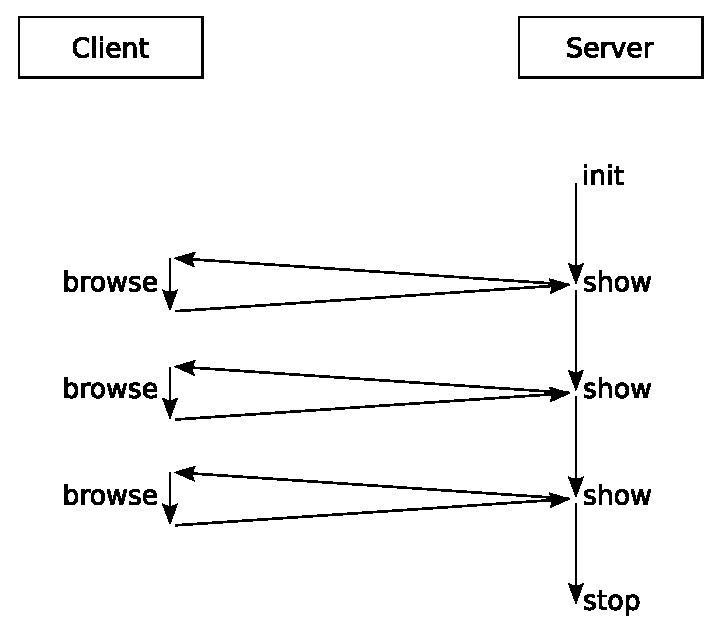
\psfig{file=figs/wig_client_and_server.eps,width=14em}
\end{center}

\vfil
\end{slide*}

\begin{slide*}
Corresponding CGI-threads:\\

\begin{center}
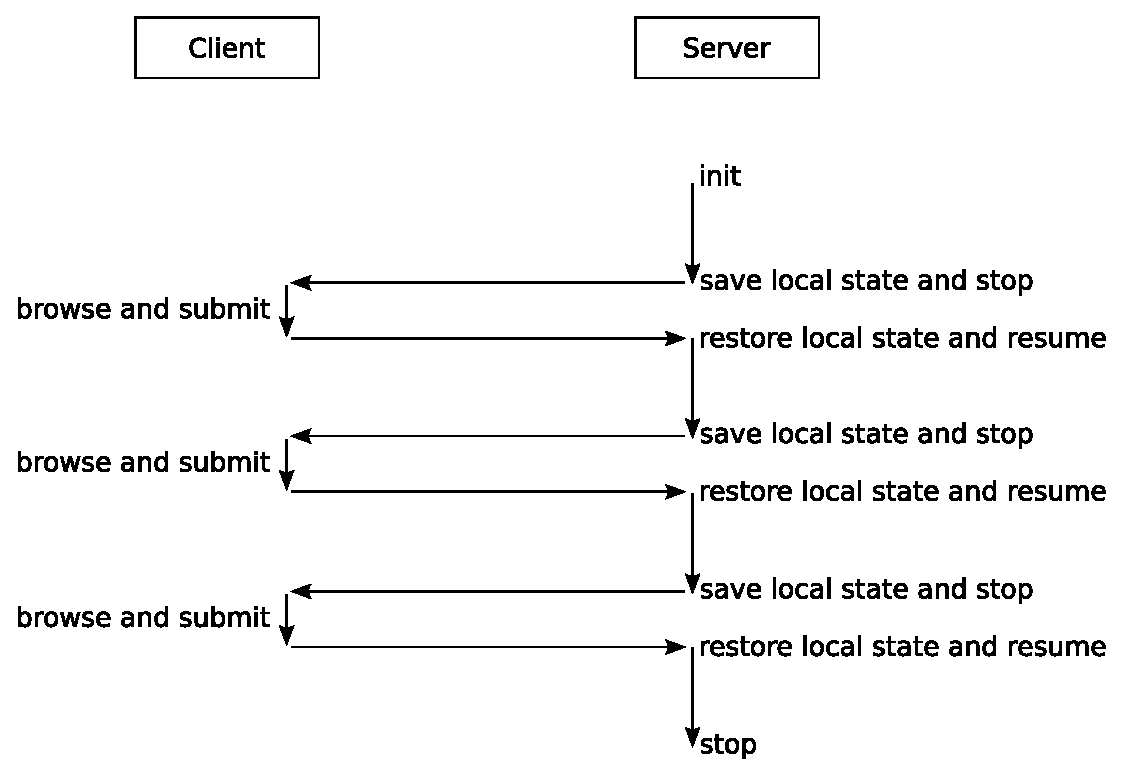
\psfig{file=figs/cgi_client_and_server.eps,width=22em}
\end{center}

\vfil
\end{slide*}
 
\begin{slide*}
Some synchronization issues and solutions:
\begin{itemize}
\item exclusive updates of global data:\\
      {\em global file locking};
\item critical sections:\\
      {\em mutex semaphores}.
\end{itemize}
\vspace*{2ex}

Some security issues and solutions:
\begin{itemize}
\item tampering with the state: \\
      {\em keep all state on the server};
\item hijacking a session:\\
      {\em use random keys in session id};
\item rolling back a thread: \\
      {\em the server has the program counter}.
\end{itemize}
\vfil
\end{slide*}
 
\begin{slide*}
A tiny WIG service:

\begin{scriptsize}
\begin{verbatim}
service {
  const html Welcome = <html> <body>
    Welcome!
  </body> </html>;

  const html Pledge = <html> <body>
    How much do you want to contribute?
    <input name="contribution" type="text" size=4>
  </body> </html>;

  const html Total = <html> <body>
    The total is now <[total]>.
  </body> </html>;

  int amount;

  session Contribute() {
     int i;
     i= 87;
     show Welcome;
     show Pledge receive[i = contribution];
     amount = amount + i;
     exit plug Total[total = amount];
  }
}
\end{verbatim}
\end{scriptsize}
\vfil
\end{slide*}
 
\begin{slide*}
Generated C-based CGI source code:
\begin{scriptsize}
\begin{verbatim}
#include <stdio.h>
#include <string.h>
#include <stdlib.h>
#include <time.h>
#include "runwig.h"

char *url;
char *sessionid;
int pc;
FILE *f;
 
void output_Welcome()
{ printf("Welcome!\n");
}

void output_Pledge()
{ printf("How much do you want to contribute?\n");
  printf("<input name=\"contribution\" 
                 type=\"text\" size=4>\n");
}

void output_Total(char *total)
{ printf("The total is now %s.\n",total);
}

int local_Contribute_i;

\end{verbatim}
\end{scriptsize}
\vfil
\end{slide*}

\begin{slide*}
\begin{scriptsize}
\begin{alltt}

\verb?int main() {?

\textit{/* initialize pseudorandom generator */}
srand48(time((time_t *)0));
\textit{/* get form fields from CGI input */}
parseFields();
\textit{/* assign the url of this service */}
url = "http://dovs-www.daimi.aau.dk/cgi-mis/tiny";
\textit{/* find current sessionid from environment */}
sessionid = getenv("QUERY_STRING");

\textit{/* do we start a new thread? */}
if (strcmp(sessionid,"Contribute")==0) 
   goto start_Contribute;
\textit{/* do we resume an old thread? */}
if (strncmp(sessionid,"Contribute$",11)==0) 
   goto restart_Contribute;
\textit{/* otherwise report an error */}
\verb?printf("Content-type: text/html\n\n");?
\verb?printf("<title>Illegal Request</title>\n");?
\verb?printf("<h1>Illegal request: %s</h1>\n",sessionid);?
exit(1);
\end{alltt}
\end{scriptsize}
\vfil
\end{slide*}

\begin{slide*}
\begin{scriptsize}
\begin{alltt}

\textit{/* start up a new thread */}
start_Contribute:
\textit{/* initialize local variables */}
local_Contribute_i = 87;
\textit{/* assign a random sessionid */}
sessionid = randomString("Contribute",20);

\textit{/* show Welcome; */}
\verb?printf("Content-type: text/html\n\n");?
\verb$printf("<form method=\"POST\" action=\"%s?%s\">\n",$
       url,sessionid);
output_Welcome();
\verb?printf("<p><input type=\"submit\" value=\"continue\">\n");?
\verb?printf("</form>\n");?
\textit{/* save local state */}
f = fopen(sessionid,"w");
\verb?fprintf(f,"1\n");?
\verb?fprintf(f,"%i\n",local_Contribute_i);?
fclose(f);
\textit{/* terminate thread */}
exit(0);
\textit{/* and resume from here */}
Contribute_1:
\end{alltt}
\end{scriptsize}
\vfil
\end{slide*}

\begin{slide*}
\begin{scriptsize}
\begin{alltt}
\textit{/* show Pledge... */}
\verb?printf("Content-type: text/html\n\n");?
\verb$printf("<form method=\"POST\" action=\"%s?%s\">\n",$
       url,sessionid);
output_Pledge();
\verb?printf("<p><input type=\"submit\" value=\"continue\">");?
\verb?printf("</form>\n");?
\textit{/* save local state */}
f = fopen(sessionid,"w");
\verb?fprintf(f,"2\n");?
\verb?fprintf(f,"%i\n",local_Contribute_i);?
fclose(f);
\textit{/* terminate thread */}
exit(0);
\textit{/* and resume from here */}
Contribute_2:

\textit{/* ...receive[i = contribution]; */}
local_Contribute_i = atoi(getField("contribution"));
\textit{/* amount = amount + i; */}
putGlobalInt("global_tiny_amount",
             getGlobalInt("global_tiny_amount")
             +local_Contribute_i);
\textit{/* exit plug Total[total = amount]; */}
\verb?printf("Content-type: text/html\n\n");?
output_Total(itoa(getGlobalInt("global_tiny_amount"))); 
exit(0);
\end{alltt}
\end{scriptsize}
\vfil
\end{slide*}

\begin{slide*}
\begin{scriptsize}
\begin{alltt}
\textit{/* restart a thread */}
restart_Contribute:
\textit{/* restore local state */}
f = fopen(sessionid,"r");
\verb?fscanf(f,"%i\n",&pc);?
\verb?fscanf(f,"%i\n",&local_Contribute_i);?
\textit{/* jump to current pc */}
if (pc==1) goto Contribute_1;
if (pc==2) goto Contribute_2;

\verb?} /* end of main () */?
\end{alltt}
\end{scriptsize}
\vfil
\end{slide*}
 
\begin{slide*}
The library {\tt runwig.h} implements:

\begin{scriptsize}
\begin{verbatim}

void parseFields();
char *getField(char *name);

char *randomString(char *name,int size);

int getGlobalInt(char *name);
void putGlobalInt(char *name,int value);

char *itoa(int i);
\end{verbatim}
\end{scriptsize}
\vfil
\end{slide*}
 
\begin{slide*}
The service can be installed by a script:

\begin{scriptsize}
\begin{verbatim}
#!/bin/sh
gcc tiny.c /path/to/wig4/runwig.c -o tiny4.cgi
cp tiny4.cgi ~/public_html/cgi-bin
chmod 755 ~/public_html/cgi-bin/tiny4.cgi
\end{verbatim}
\end{scriptsize}

and invoked by:

\begin{scriptsize}
\begin{verbatim}
http://www.cs.mcgill.ca/~`whoami`/cgi-bin/tiny.cgi?Contribute
\end{verbatim}
\end{scriptsize}

\vspace{0.5in}
Are we having fun yet?
\vfil
\end{slide*}
 
\end{document}
